\subsection{Model Definition}
\label{sec:setup.arch.definition}

The archetypal model is defined as the map $x_{n+1} = f(x_n) \mod 1$ where $f$ is given by the following set of equations.
\begin{align}
	f(x) & = \begin{cases}
		         g(x)                             & \text{if } x < \frac{1}{2} \\
		         g(x - \frac{1}{2}) + \frac{1}{2} & \text{else}
	         \end{cases} \label{equ:arch.f}           \\
	g(x) & = \begin{cases}
		         g_L(x) = a_L \cdot x^2 + b_L \cdot x + c_L & \text{if } x < \frac{1}{4} \\
		         g_R(x) = b_R \cdot x + c_R                 & \text{else}
	         \end{cases} \label{equ:arch.g}
\end{align}

\subsection{Parameters}
\label{sec:setup.arch.parameters}

Since the function $g_R$ is now linear, only two \hl{composite} parameters are necessary to control the shape of the branches $f_\B$ and $f_\D$.
The chosen \hl{composite} parameters are $g_R\left(\frac{1}{4}\right)$ and $g_R\left(\frac{1}{2}\right)$ and the \hl{composite} parameter $\left. \frac{d}{dx} g_R(x) \right|_{x = \frac{1}{2}}$ used in the previous sections is not used.
As before, the value of the \hl{composite} parameter $g_R\left(\frac{1}{2}\right) = \frac{1}{2} + \frac{1}{40}$ is fixed to be just above the bisector $y = x$, and the \hl{composite} parameter $g_R\left(\frac{1}{4}\right)$ is varied.

\begin{subequations}
	\begin{align}
		g_R\left(\frac{1}{4}\right) & = \frac{b_R}{4} + c_R \label{equ:setup.arch.A} \\
		g_R\left(\frac{1}{2}\right) & = \frac{b_R}{2} + c_R \label{equ:setup.arch.B}
	\end{align}
\end{subequations}

\Cref{equ:setup.arch.A,equ:setup.arch.B} are the equations for the values of $g_R\left(\frac{1}{4}\right)$ and $g_R\left(\frac{1}{2}\right)$.
This is a system of equations that needs to be solved for the parameters $b_R$ and $c_R$.
As before, this is achieved by writing the system of equations as a matrix and computing the inverse matrix.
\Cref{equ:setup.arch.matrix} demonstrates this.

\begin{align}
	\begin{pmatrix}
		\frac{1}{4} & 1 \\
		\frac{1}{2} & 1
	\end{pmatrix}^{-1} & =
	\begin{pmatrix}
		-4 & 4  \\
		2  & -1
	\end{pmatrix}
	\label{equ:setup.arch.matrix}
\end{align}

Hence, the equations for $b_R$ and $c_R$ in dependence of the \hl{composite} parameters $g_R\left(\frac{1}{4}\right)$ and $g_R\left(\frac{1}{4}\right)$ are \Cref{equ:setup.arch.bR,equ:setup.arch.cR}.

\begin{align}
	b_R & = -4 \cdot g_R\left(\frac{1}{4}\right) + 4 \cdot g_R\left(\frac{1}{2}\right) \label{equ:setup.arch.bR} \\
	c_R & = 2 \cdot g_R\left(\frac{1}{4}\right) - 1 \cdot g_R\left(\frac{1}{2}\right) \label{equ:setup.arch.cR}
\end{align}



As mentioned before, the parameter $\alpha$ is \hl{given a negative sign} to mirror the \gls{pi} structure.
So $\alpha = -g_R\left(\frac{1}{4}\right)$ in the archetypal model.
All parameters are listed in \Cref{table:setup.arch.parameters} a for better overview.

\begin{table}
	\centering
	\begin{tabular}{|c|c|}
		\hline
		Model Parameter               & Value                                                                       \\ \hline \hline
		$a_L$                         & $4$                                                                         \\ \hline
		$b_L$                         & $-\frac{1}{2}$                                                              \\ \hline
		$c_L$                         & $\beta$                                                                     \\ \hline \hline
		$b_R$                         & $4 \cdot g_R\left(\frac{1}{2}\right) - 4 \cdot g_R\left(\frac{1}{4}\right)$ \\ \hline
		$c_R$                         & $2 \cdot g_R\left(\frac{1}{4}\right) - g_R\left(\frac{1}{2}\right)$         \\ \hline
		$g_R\left(\frac{1}{4}\right)$ & $-\alpha$                                                                   \\ \hline
		$g_R\left(\frac{1}{2}\right)$ & $\frac{1}{2} + \frac{1}{40}$                                                \\ \hline
	\end{tabular}
	\caption[Overview of parameters of the archetypal model]{
		Overview of the parameter values of all parameters of the archetypal model with the \hl{composite} parameters $g_R\left(\frac{1}{4}\right)$ and $g_R\left(\frac{1}{2}\right)$.
		In the top part, there are all parameters of the function $g_L$, and in the bottom part are the parameters of the function $g_R$.
	}
	\label{table:setup.arch.parameters}
\end{table}

\subsection{Parameter Effects}
\label{sec:setup.arch.parameterfx}

The effects of the defined parameters on the model function are straightforward and can be read directly from the previous section.
In summary, the parameter $\alpha$ changes the values of the model function on the left sides of the branches $f_\B$ and $f_\D$.
Where a lower value of $\alpha$ means a higher value of the model function in those regions, because the parameter \hl{has negative sign}.
In the previously defined notation, this is written as $\AL_{\B}^-$.
This notation is defined in \Cref{sec:setup.char.paramfx}.
The parameter $\beta$ changes the values of the model function on the whole branches $f_\A$ and $f_\C$.
A higher $\beta$ means higher values, and it is written as $\AW_{\A}^+$.

\Cref{fig:setup.arch.paramfx} illustrates these parameter effects.
Both figures show the model function for three parameter values, where either $\alpha$ or $\beta$ is fixed, and the other parameter is varied.
The model functions are labeled according to the value of the variable parameter, $f^L$ for the lowest value, $f^M$ for the middle value, and $f^H$ for the highest value.
\Cref{fig:setup.arch.paramfx.alpha} illustrates the effect of $\alpha$.
One can see, how the values of the model function at the left borders of branches $f_\B$ and $f_\D$ are smaller for higher values of $\alpha$.
\Cref{fig:setup.arch.paramfx.beta} illustrates the effect of $\beta$.
Here one can see, how the values of the model function for the whole branches $f_\A$ and $f_\C$ increase for larger values of $\beta$.

\begin{figure}
	\centering
	\subfloat[$\alpha$]{
		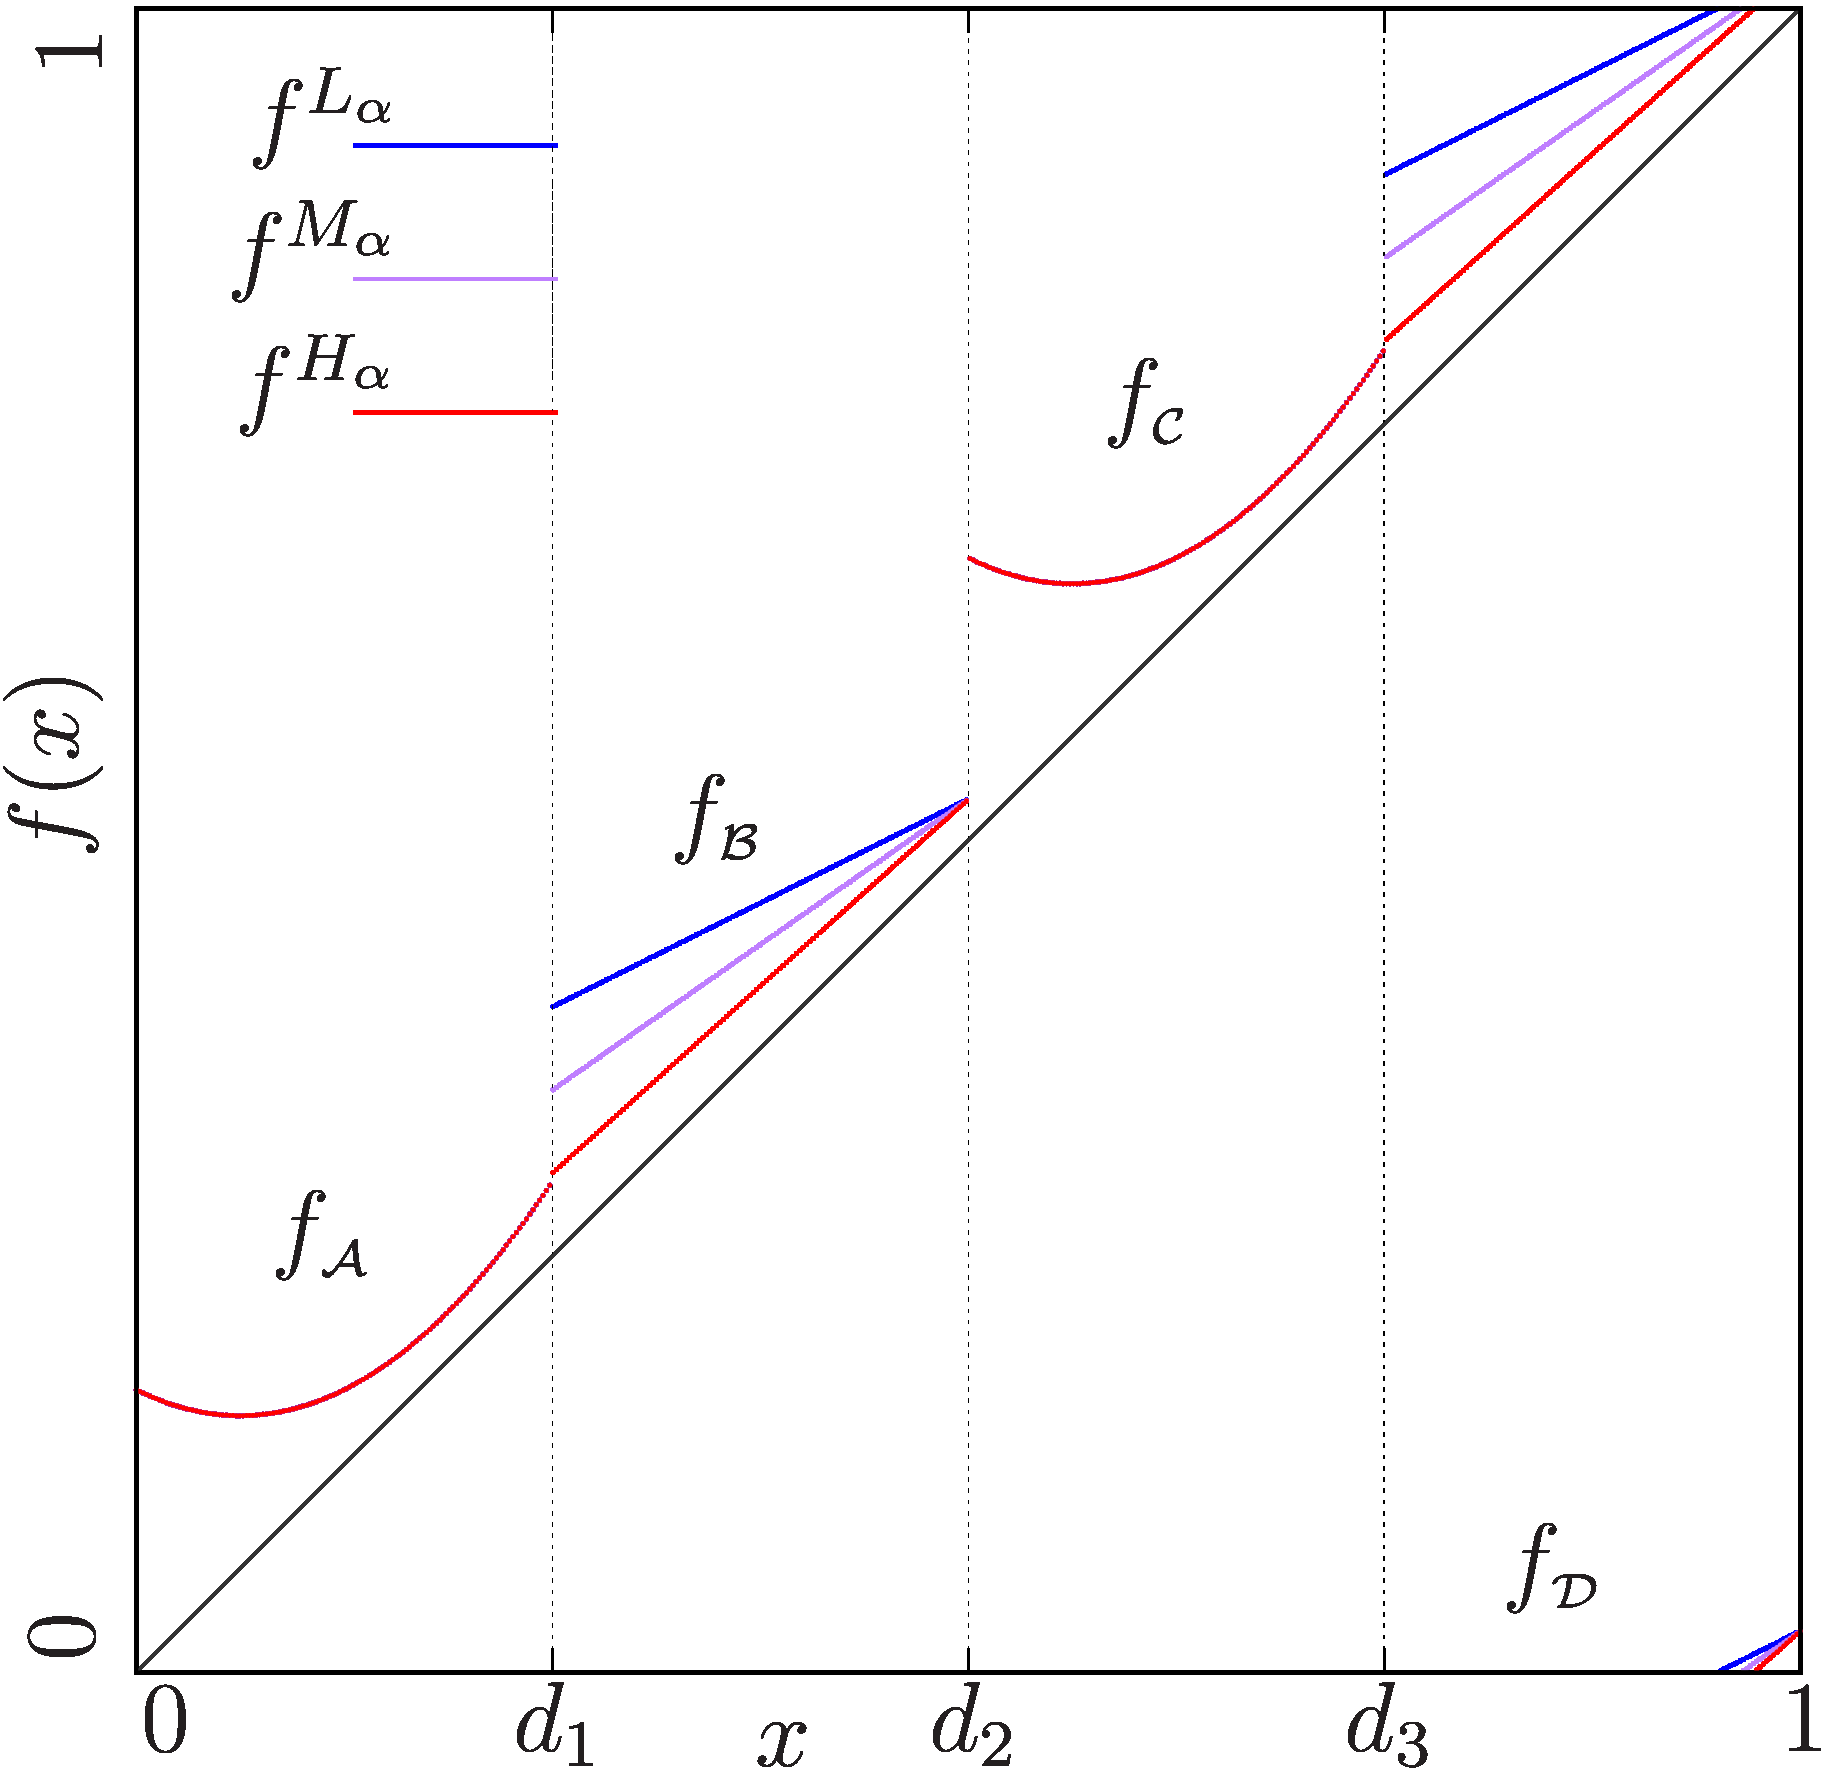
\includegraphics[width=.4 \textwidth]{../Figures/5/5.13a/illustration.png}
		\label{fig:setup.arch.paramfx.alpha}
	}
	\subfloat[$\beta$]{
		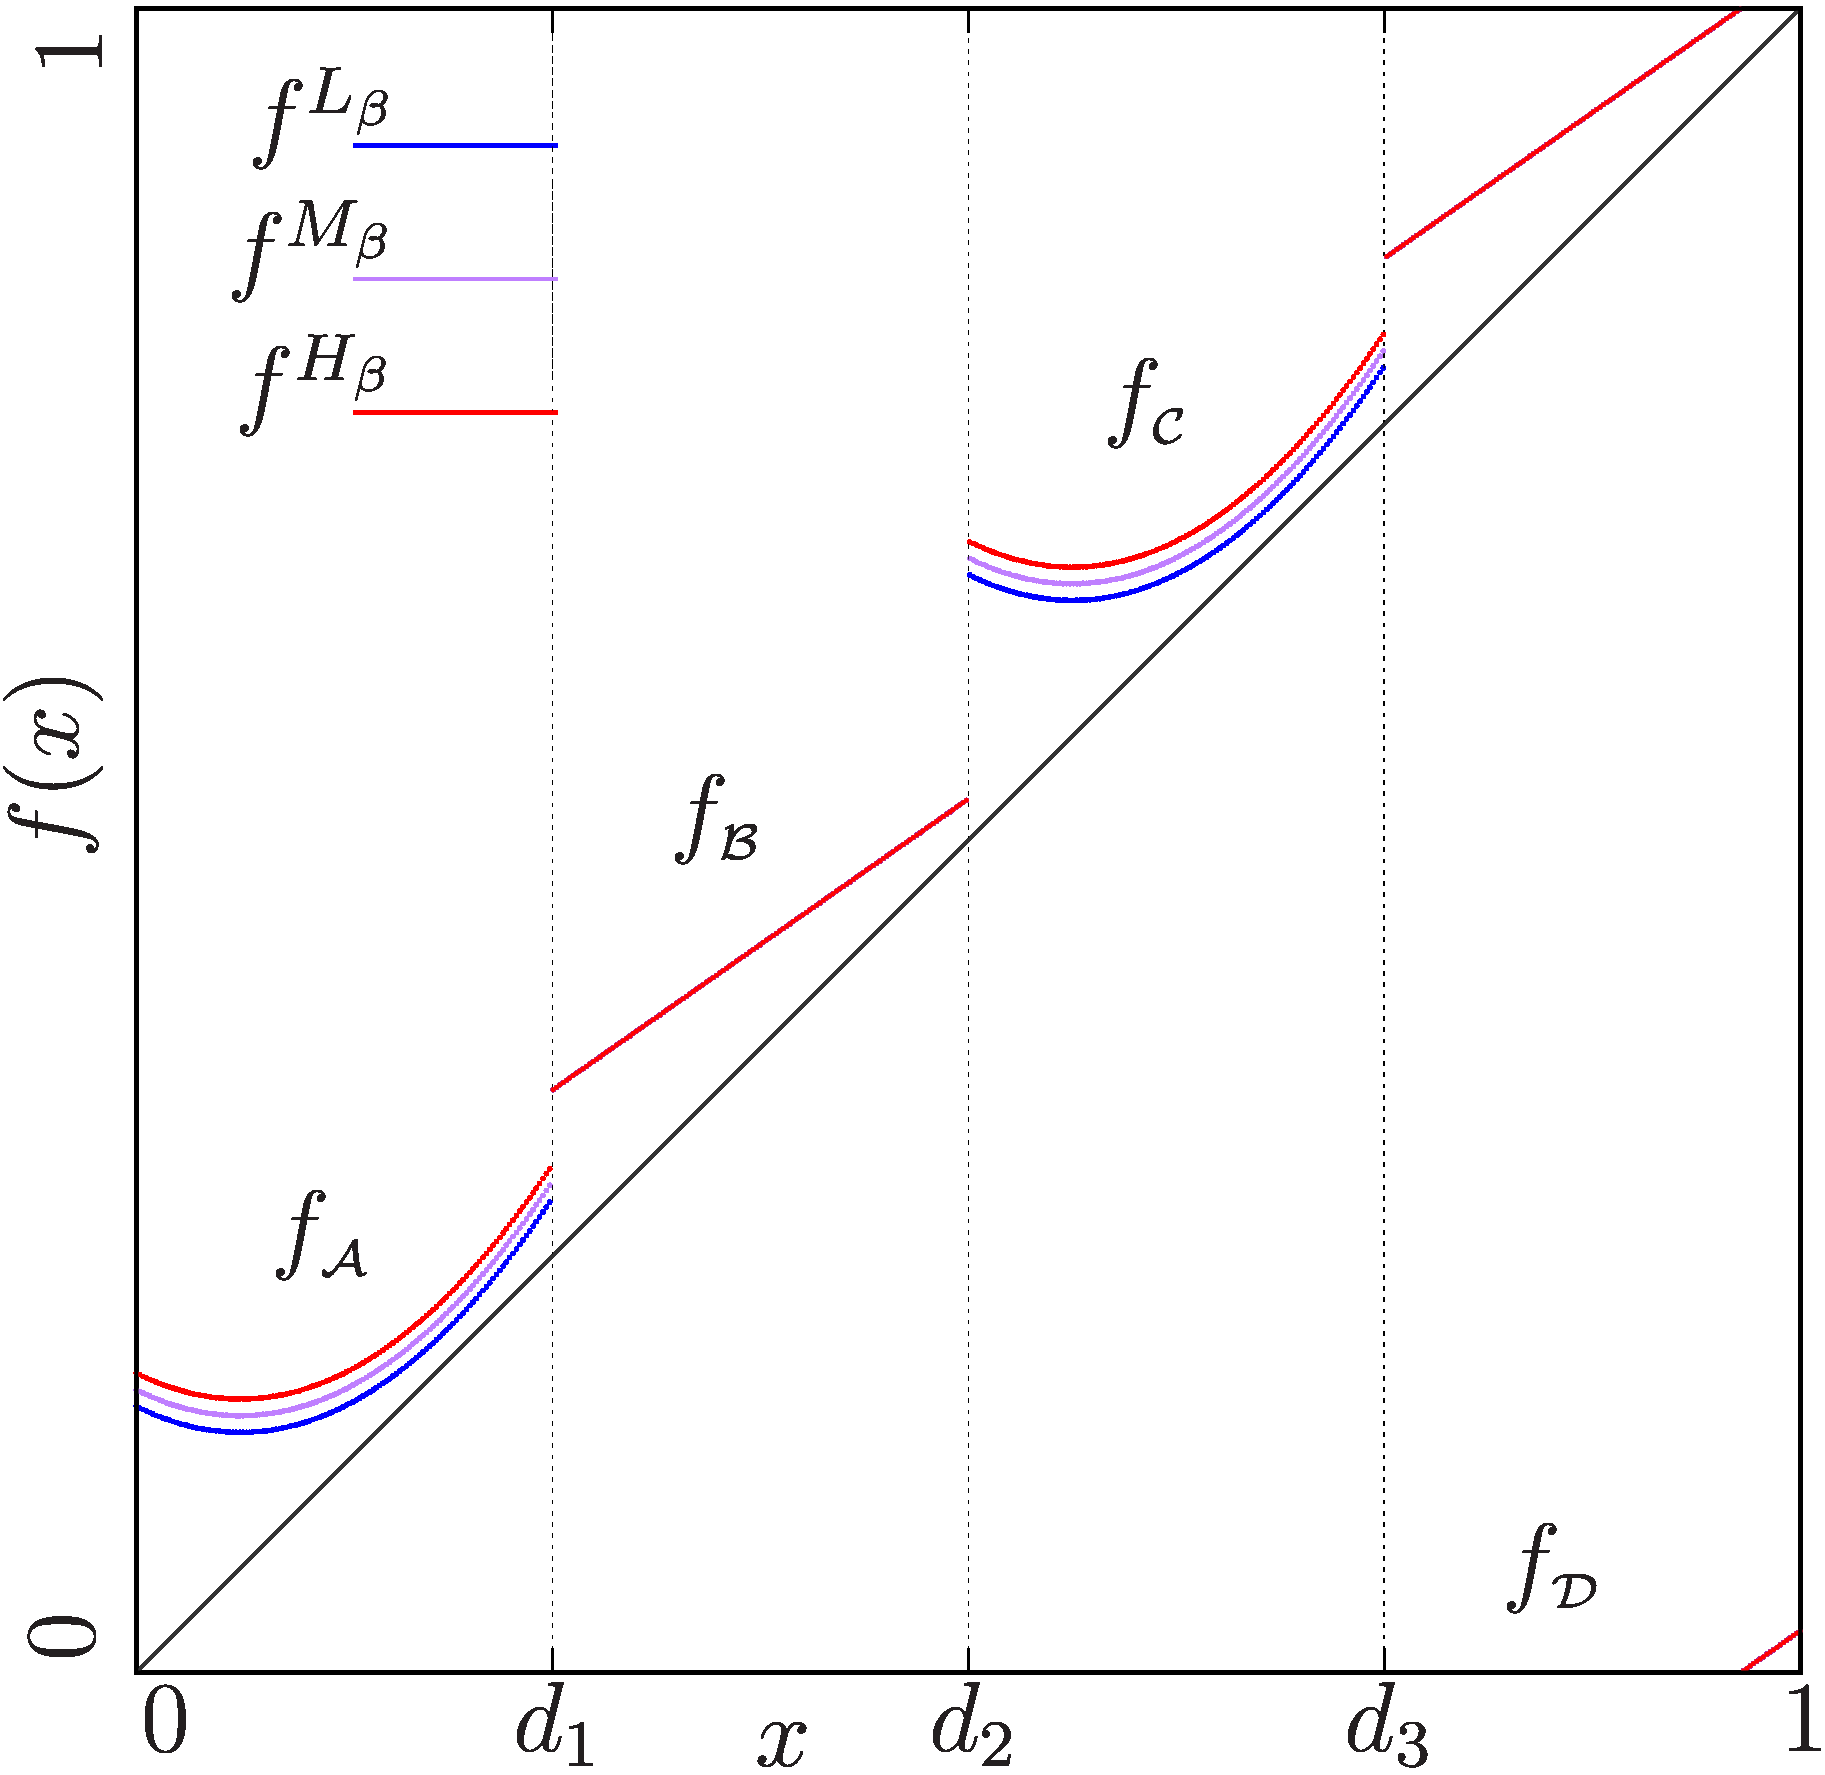
\includegraphics[width=.4 \textwidth]{../Figures/5/5.13b/illustration.png}
		\label{fig:setup.arch.paramfx.beta}
	}
	\caption[The effects of single parameters on the piecewise hybrid quadratic model function]{
		The effects of varying the parameters $\alpha$ and $\beta$ alone on the piecewise hybrid quadratic model function.
		(a) shows the effects of $\alpha$ on the model function with fixed $\beta = 0.17$.
		The function $f^{L\alpha}$ is for $\alpha = -0.4$, $f^{M_\alpha}$ is for $\alpha = -0.35$, and $f^{H_\alpha}$ is for $\alpha = -0.3$.
		(b) shows the effects of $\beta$ on the model function with fixed $\alpha = -0.35$.
		The function $f^{L_\beta}$ is for $\beta = 0.16$, $f^{M_\beta}$ is for $\beta = 0.17$, and $f^{H_\beta}$ is for $\beta = 0.18$.
	}
	\label{fig:setup.arch.paramfx}
\end{figure}

\Cref{table:setup.arch.paramfx} lists the effects of parameters $\alpha$ and $\beta$ in a table, like also done for the original model in \Cref{sec:setup.char.paramfx}.
Additionally, the parameter effects of the parameters in the original model are listed for comparison.
This gives a nice overview of which characteristics of the original model function are necessary for the observed bifurcation structure.
Especially it shows, which parameter effects are not necessary.
For example, the effect $\AMi_{\B}^{L-}$ cannot even be fabricated in this model since branches $\Branch_\B$ and $\Branch_\D$ are linear and do not have a local minimum.
Also, the effect $\AB_{\B\C}^L$, which is the movement of the borders between branches $\Branch_\B$ and $\Branch_\C$ (and $\Branch_\D$ and $\Branch_\A$ respectively), is not necessary.

\begin{table}
	\centering
	\begin{tabular}{|c||c|c||c|c|} \hline
		Combined         & $E_0$            & $\chi_0$          & $\alpha$     & $\beta$        \\ \hline \hline
		$\AL_{\B}^{-}$   & $\AL_{\B}^{-}$   &                   & $\AL_{\B}^-$ &                \\ \hline
		$\AMi_{\B}^{L-}$ & $\AMi_{\B}^{L-}$ & $-\AMi_{\B}^{+}$  &              &                \\ \hline
		$\AW_{\A}^{+}$   &                  & $\AW_{\A}^{+}$    &              & $\AW_{\A}^{+}$ \\ \hline \hline
		$\AB_{\B\C}^{L}$ &                  & $\AB_{\B\C}^{L}$  &              &                \\ \hline
		                 & $\AB_{\A\B}^{R}$ & $-\AB_{\A\B}^{L}$ &              &                \\ \hline
	\end{tabular}
	\caption[Comparison table of parameter effects in the piecewise hybrid quadratic model and the original model]{
		Comparison table of the parameter effects of $E_0$ and $\chi_0$ in the original model and the effects of $\alpha$ and $\beta$ in the piecewise hybrid quadratic model.
		Each effect of the parameters $E_0$ and $\chi_0$ as listed in \Cref{table:setup.char.paramfx} is also listed here.
		If $\alpha$ or $\beta$ cause the same effect, it is also listed in the respective column.
	}
	\label{table:setup.arch.paramfx}
\end{table}
